\documentclass[a4paper]{report}

\usepackage{amsmath,amssymb,stmaryrd,latexsym}
\usepackage{titlepic}
\usepackage{syntax}
\usepackage{alltt}
\usepackage{graphicx}   % Including Graphics
%\usepackage{verbatim} 
\usepackage{spverbatim}
\usepackage{alltt} 
\usepackage{xspace} 
\usepackage{listings} 
\usepackage{ifthen}
\usepackage{adjustbox}
\usepackage{xhfill}% http://ctan.org/pkg/xhfill
\usepackage{color}
\usepackage{fancybox}
\usepackage{fancyvrb}
\usepackage{fixltx2e}
\usepackage[multiple]{footmisc}
\usepackage{grammar-defns}  %% Generated by Obelisk

\newsavebox{\FVerbBox}
\newenvironment{FVerbatim}
 {\VerbatimEnvironment
  \begin{center}
  \begin{lrbox}{\FVerbBox}
  \begin{BVerbatim}}
 {\end{BVerbatim}
  \end{lrbox}
  \fbox{\usebox{\FVerbBox}}
  \end{center}}

\newboolean{devel}
\setboolean{devel}{false}

\lstloadlanguages{C++,VHDL}
\lstset{frameround=tttt} 
\lstset{captionpos=t}
\lstset{breaklines=true}
\lstset{escapechar=@}
%\lstset{aboveskip=2\medskipamount}
%\lstset{belowskip=1.5\medskipamount}
%\lstset{abovecaptionskip=\medskipamount}
\lstdefinelanguage{Rfsm}{keywords={type,enum,record,function,return,fsm,model,in,out,inout,vars,states,trans,itrans,on,when,with,periodic,sporadic,value_changes,event,bool,input,output,shared},morecomment=[l]{--}}
\lstdefinelanguage{ctask}{language=C,morekeywords={task,wait_ev,wait_evs,notify_ev,in,out,inout}}
\lstdefinelanguage{systemc}{language=C++,morekeywords={SC_MODULE,SC_METHOD,SC_THREAD,sc_in,sc_out,sc_inout}}

%%% Better hyphenation:
%\sloppy
\setlength{\topmargin}{0pt}
\setlength{\oddsidemargin}{0pt}
\setlength{\textheight}{600pt}
\setlength{\textwidth}{448pt}

%\Newcommand{\docdate}{\today} %%%!!!!
\newcommand{\step}{\medskip$\blacktriangleright$\xspace}

\newcommand{\version}{1.6}

\newcommand{\ie}{\emph{i.e.}\xspace}
\newcommand{\txt}[1]{\hbox{#1}}
\newcommand{\emtxt}[1]{\hbox{\em{#1}}}
\newcommand{\bftxt}[1]{\hbox{\bf{#1}}}
\ifthenelse{\boolean{devel}}{\newcommand{\note}[1]{\marginpar{\tiny #1}}}{\newcommand{\note}[1]{}}
\newcommand{\todo}[1]{\note{TODO: #1}}
\ifthenelse{\boolean{devel}}{\newcommand{\tbw}[1]{$\spadesuit$ {\bf To be written\ldots}\xspace}}{\newcommand{\tbw}[1]{}}
\ifthenelse{\boolean{devel}}{\newcommand{\tbc}[1]{$\spadesuit$ {\bf To be continued\ldots}\xspace}}{\newcommand{\tbc}[1]{}}

\newcommand{\rfsm}{RFSM\xspace}
\newcommand{\ocaml}{{\sc Objective Caml}\xspace}

\newcommand{\example}[1]{\fcolorbox{white}{lightgray}{#1}}
\newcommand{\ifname}[3]{$\mathtt{#1}_{\mathtt{#2}}\mathtt{#3}$}

%\newenvironment{example}{\medskip\noindent{\it Example :}\begin{alltt}}{\end{alltt}}

\title{RFSM User Manual - \version}

\author{J. S\'erot}

\titlepic{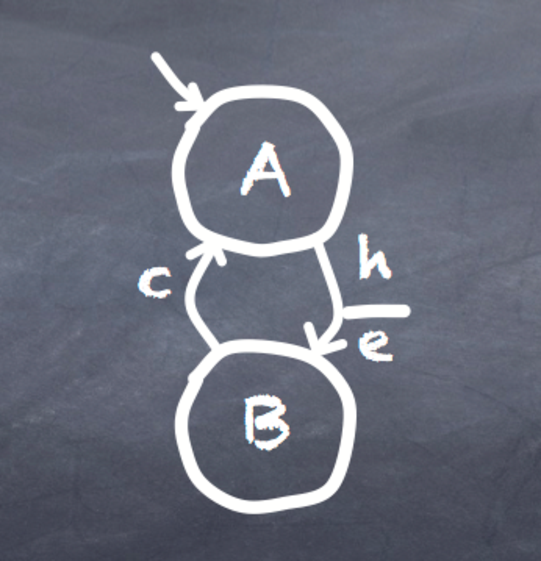
\includegraphics[width=0.5\textwidth]{figs/rfsm-logo}}
\date{}

\begin{document}

\maketitle

%\tableofcontents

\section{Introduction}
\label{sec:intro}

Algebraic data types (ADT) are an important tool in functional programming which deliver a way to represent flexible and easy to manipulate data structures.
To inspect the contents of an ADT's values a generic construct~--- \emph{pattern matching}~--- is used. The importance of pattern matching efficient
implementation stimulated the development of various advanced techniques which provide good results in practice. The objective of our work is to use these
results as a baseline for a case study of relational synthesis\footnote{We have to note that this term is overloaded and can be used to refer to completely
different approaches than we utilize.}~--- an approach for program synthesis based on application of relational programming~\cite{TRS,WillThesis}, and,
in particular, relational interpreters~\cite{unified} and relational conversion~\cite{conversion}. Relational programming can be considered as a specific form
of constraint logic programming centered around \textsc{miniKanren}\footnote{\url{http://minikanren.org}}, a combinator-based DSL, implemented for a number of host languages.
Unlike \textsc{Prolog}, which employs a deterministic depth-first search, \textsc{miniKanren} advocates a 
%completely 
more
declarative approach, in which a user is not
allowed to rely on a concrete search discipline, which means, that the specifications, written in \textsc{miniKanren}, are understood much more symmetrically.
The distinctive feature of \textsc{miniKanren} is complete \emph{interleaving search}~\cite{search}. The basic constraint is unification with occurs check, although
advanced implementations support other primitive constructs, such as disequality or finite-domain constraints~\cite{CKanren}. Syntactically, \textsc{miniKanren} is mutually
convertible to \textsc{Prolog}, but, unlike latter, makes use of explicit logical connectives (conjunction and disjunction), existential quantification and unification.
 
A distinctive application of relational programming is implementing \emph{relational interpreters}~\cite{Untagged}. Unlike conventional interpreters, which for a program and
input value produce output, relational interpreters can operate in various directions: for example, they are capable of computing an input value for a given
program and a given output, or even synthesize a program for a given pairs of input-output values. The latter case forms a basis for program synthesis~\cite{eigen,unified}.

Our approach is based on relational representation of the source language pattern matching semantics on the one hand, and
the semantics of the intermediate-level implementation language on the other. We formulate the condition necessary for a correct and complete implementation of pattern matching and use it to
construct a top-level goal which represents a search procedure for all correct and complete implementations. We also present a number of techniques which make it possible to come up with an
\emph{optimal} solution as well as optimizations to improve the performance of the search. Similarly to many other prior works we use the size of the synthesized code, which can be measured
statically, to distinguish better programs. Our implementation\footnote{\url{https://github.com/Kakadu/pat-match/tree/aplas2020}} makes use of \textsc{OCanren}\footnote{\url{https://github.com/JetBrains-Research/OCanren}}~---
 a typed implementation of \textsc{miniKanren} for \textsc{OCaml}~\cite{OCanren}, and \textsc{noCanren}\footnote{\url{https://github.com/Lozov-Petr/noCanren}}~--- 
a converter from the subset of plain \textsc{OCaml} into \textsc{OCanren}~\cite{conversion}. An initial  evaluation, performed for a set of benchmarks taken from other papers, showed our synthesizer performing well.
However, being aware of some pitfalls of our approach, we came up with a set of counterexamples on which it did not provide any results in observable time, so we do not consider the problem
completely solved. We also started to work on mechanized 
formalization\footnote{\url{https://github.com/dboulytchev/Coq-matching-workout}},
written in \textsc{Coq}~\cite{Coq}, to make the justification of our approach more solid and easier to verify, but this formalization is not yet complete. 

 

\begin{comment}
We apply relational programming techniques to the problem of synthesizing efficient implementation for a pattern matching construct.
Although in principle pattern matching can be implemented in a trivial way, the result suffers from inefficiency in terms of both
performance and code size. Thus, in implementing functional languages alternative, more elaborate  approaches are widely used.
However, as there are multiple kinds and flavors of pattern matching constructs, these approaches have to be specifically developed
and justified for each concrete inhabitant of the pattern matching ``zoo''. We formulate the pattern matching synthesis problem in
declarative terms and apply relational programming, a specific form of constraint logic programming, to develop a 
develop optimizations which improve the efficiency of the synthesis and guarantee the
optimality of the result. 
\end{comment}

\chapter{Overview}
\label{cha:overview}

This chapter gives informal introduction to the RFSM language and of how to use it to describe 
FSM-based systems.

\medskip
Listing~\ref{lst:rfsm-gensig} is an example of a simple RFSM program\footnote{This program is
  provided in the distribution, under directory \texttt{examples/single/gensig/v2}.}. This program is
used to describe and simulate the model of a calibrated pulse generator. Given an input clock
\verb|H|, with period $T_H$, it generates a pulse of duration $n \times T_H$ whenever input
\texttt{E} is set when event $H$ occurs.

\begin{lstlisting}[language=Rfsm,frame=single,numbers=left,caption=A simple RFSM
  program,label={lst:rfsm-gensig},float]
@\label{gensig-1a}@fsm model gensig <n: int> (
  in h: event,
  in e: bool,
  out s: bool)
{
@\label{gensig-1}@  states: E0 where s=0, E1 where s=1;
  states: E0, E1;
@\label{gensig-3}@  vars: k: int<0:n>;
  trans:
  | E0 -> E1 on h when e=1 with k:=1
@\label{gensig-4}@  | E1 -> E1 on h when k<n with k:=k+1
@\label{gensig-5}@  | E1 -> E0 on h when k=n;
  itrans:
  | -> E0;
@\label{gensig-1b}@}

@\label{gensig-2a}@input H : event = periodic (10,0,80)
input E : bool = value_changes (0:0, 25:1, 35:0)
@\label{gensig-2b}@output S : bool 

@\label{gensig-6}@fsm g = gensig<4>(H,E,S)
\end{lstlisting}

The program can be divided in four parts.

\medskip The first part (lines \ref{gensig-1a}--\ref{gensig-1b}) gives a \textbf{generic model} of
the generator behavior. The model, named \verb|gensig|, has one parameter, \verb|n|, two inputs,
\verb|h| and \verb|e|, of type \verb|event| and \verb|bool| respectively, and one output \verb|s| of
type \verb|bool|. Its behavior is specified as a reactive FSM with two states, \verb|E0| and
\verb|E1|, and one internal variable \verb|k|. The transitions of this FSM are given after the
\verb|trans:| keyword in the form :
\begin{center}
  \framebox{\lstinline[language=Rfsm]{| source_state -> destination_state on ev when guard with actions}}
\end{center}
where
\begin{itemize}
\item \emph{ev} is the event trigerring the transition,
\item \emph{guard} is a set of (boolean) conditions,
\item \emph{actions} is a set of actions performed when the transition is enabled.
\end{itemize}

The semantics is that the transition is enabled
whenever the FSM is in the source state, the event \emph{ev} occurs and all the conditions in the
guard are true. The associated actions
are then performed and the FSM moves to the destination state. For example, the first transition is
enabled whenever an event occurs on input \verb|h| and, at this instant, the value of input \verb|e|
is 1. The FSM then goes from state \verb|E0| to state \verb|E1| and sets its internal variable 
\verb|k|.
   
The \emph{initial transition} of the FSM is given 
after the \verb|itrans:| keyword in the form :
\begin{center}
  \framebox{\lstinline[language=Rfsm]{| -> initial_state with actions}}
\end{center}
Here the FSM is initially in state \verb|E0|.

The value of the \texttt{s} output is attached to states, using
the \lstinline[language=Rfsm]{where} keyword~: this value is 0 when the
system is in state \texttt{E0} and 1 when the system is in state \texttt{E1}.

\textbf{Note}. In the transitions, the \lstinline[language=Rfsm]{when guard} and
\lstinline[language=Rfsm]{with actions} are optional and may be omitted.

A graphical representation of the \verb|gensig| model is given in
Fig.~\ref{fig:rfsm-gensig-model} (this representation was actually automatically generated from the
program in Listing~\ref{lst:rfsm-gensig}, as explained in Chap.~\ref{cha:rfsmc}). 

\begin{figure}[!h]
   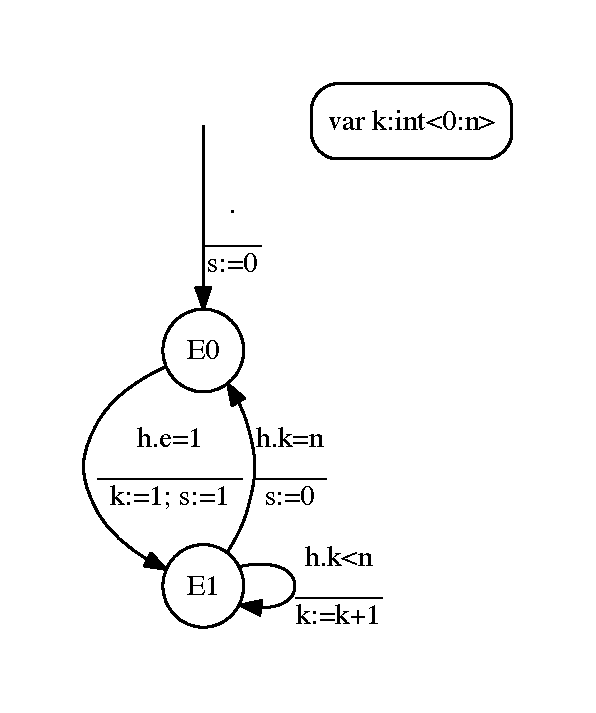
\includegraphics[height=8cm]{figs/gensig-model}
   \centering
  \caption{A graphical representation of FSM model defined in Listing~\ref{lst:rfsm-gensig}}
  \label{fig:rfsm-gensig-model}
\end{figure}

Note that, at this level, the value of the parameter \verb|n|, used in the type of the internal
variable \verb|k| (line~\ref{gensig-3}) and in the transition conditions (lines \ref{gensig-4} and
\ref{gensig-5}) is left unspecified, making the \verb|gensig| model a \emph{generic} one.

\medskip The second part of the program (lines \ref{gensig-2a}--\ref{gensig-2b}) lists \textbf{global inputs and
  outputs}\footnote{In case of multi-FSM programs, this part will also contains the declaration of
  \emph{shared} events and variables. See Sec.~\ref{sec:globals}.}.  For global outputs the
declaration simply gives a name and a type.  For global inputs, the declaration also specifies the
\textbf{stimuli} which are attached to the corresponding input for simulating the system. The
program of Listing~\ref{lst:rfsm-gensig} uses two kinds of stimuli\footnote{See
  Sec.~\ref{sec:globals} for a complete description of stimuli.}. The stimuli attached to input
\verb|H| are declared as \emph{periodic}, with a period of 10 time units, a start time of 0 and a
end time of 80. This means than an event will be produced on this input at time 0, 10, 20, 30, 40,
50, 60, 70 and 80. The stimuli attached to input \verb|E| say that this input will respectively take
value 0, 1 and 0 at time 0, 25 and 35 (thus producing a ``pulse'' of duration 10 time units starting
at time 25).

\medskip
The third and last part of the program (line~\ref{gensig-6}) consists in building the global model of the system by
\emph{instanciating} the FSM model(s).
Instanciating a model creates a ``copy'' of this model for which
\begin{itemize}
\item the generic parameters (\verb|n| here) are now bound to actual values (4 here),
\item the inputs and outputs are connected to the global inputs or outputs. 
\end{itemize}

\medskip
A graphical representation of the system described in Listing~\ref{lst:rfsm-gensig} is given in
Fig.~\ref{fig:rfsm-gensig-top}\footnote{Again, this representation was actually automatically generated from the
program in Listing~\ref{lst:rfsm-gensig}, as explained in Chap.~\ref{cha:rfsmc}}. 

\begin{figure}[!h]
   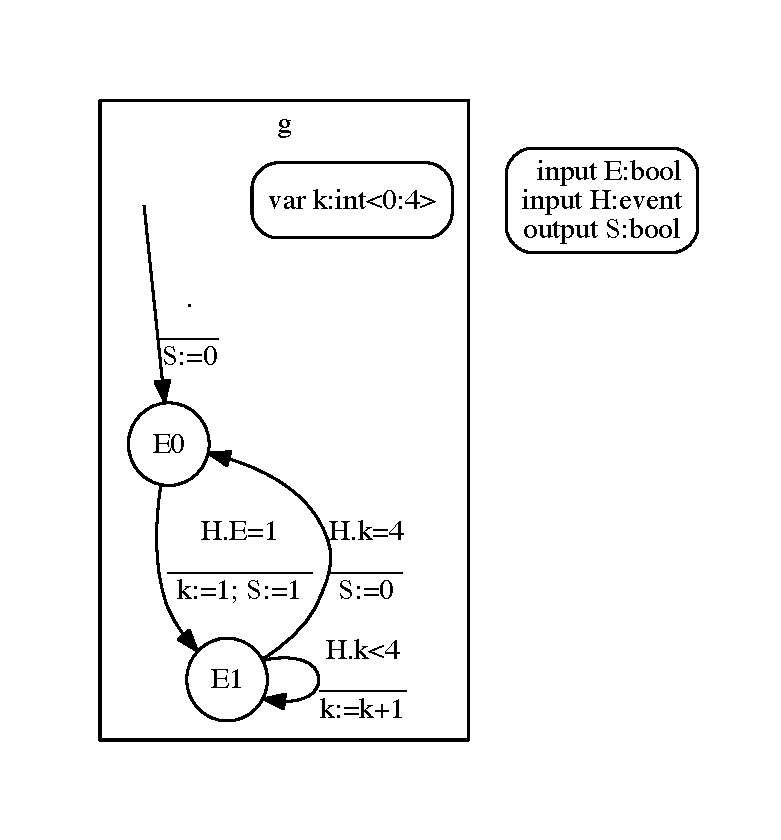
\includegraphics[height=8cm]{figs/gensig-top}
   \centering
  \caption{A graphical representation of system described in Listing~\ref{lst:rfsm-gensig}}
  \label{fig:rfsm-gensig-top}
\end{figure}

\section*{Simulating}
\label{sec:simulating-1}

Simulating the program means computing the reaction of the system to the input stimuli. Simulation
can be performed the RFSM command-line compiler or the IDE (see Chap.~\ref{cha:rfsmc} and \ref{cha:gui} resp.).
It produces a set of
\emph{traces} in VCD (Value Change Dump) format which can visualized using \emph{waveform viewers}
such as \texttt{gtkwave}. The simulation results for the program in Listing~\ref{lst:rfsm-gensig}
are illustrated in Fig.~\ref{fig:rfsm-gensig-chrono}.

\begin{figure}[!h]
   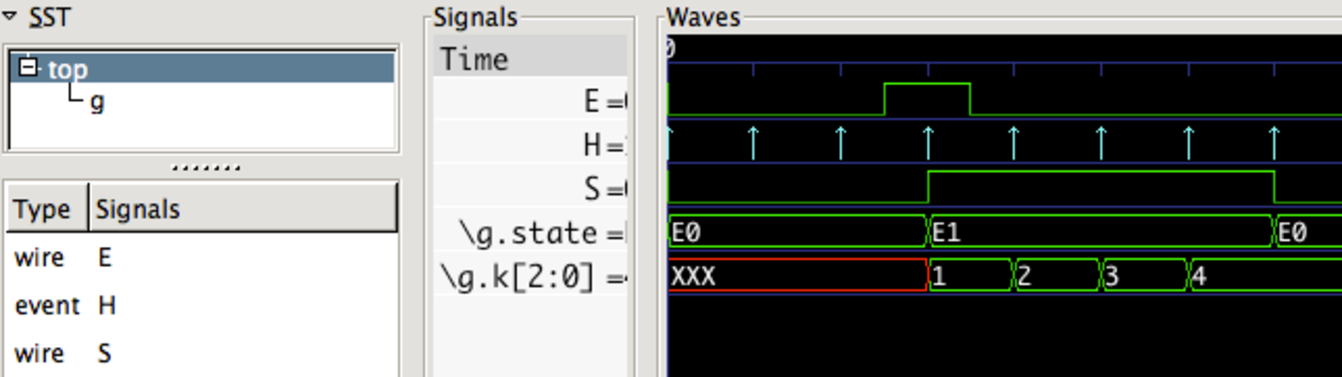
\includegraphics[width=\textwidth]{figs/gensig-chrono}
   \centering
  \caption{Simulation results for the program in Listing~\ref{lst:rfsm-gensig}, viewed using
    \texttt{gtkwave}}
  \label{fig:rfsm-gensig-chrono}
\end{figure}

\section*{Code generation}
\label{sec:code-generation-1}

RFSM can also generate code implementing the described systems simulation and/or
integration to existing applications.

\medskip
Currently, three backends are provided :
\begin{itemize}
\item a backend generating a C-based implementation of each FSM instance,
\item a backend generating a \emph{testbench} implementation in SystemC (FSM instances + stimuli
  generators),
\item a backend generating a \emph{testbench} implementation in VHDL (FSM instances + stimuli
  generators).
\end{itemize}

\medskip
The target language for the C backend is a C-like language augmented with
\begin{itemize}
\item a \verb|task| keyword for naming generated behaviors,
\item \verb|in|, \verb|out| and \verb|iinout| keywords for identifying inputs and outputs,
\item a builtin \verb|event| type,
\item primitives for handling events : \verb|wait_ev()|, \verb|wait_evs()| and
  \verb|notify_ev()|. 
\end{itemize}
The idea is that the generated code can be turned into an application for a multi-tasking operating
system by providing actual implementations of the corresponding constructs and primitives.

\medskip
For the SystemC and VHDL backends, the generated code can actually be compiled and executed for
simulation purpose and. The FSM implementations generated by the VHDL backend can also be
synthetized to be implemented hardware using hardware-specific tools\footnote{We use the
  \textsc{quartus} toolchain from Intel/Altera.}. 

\medskip
Appendices C1, C2 and C3 respectively give the C and SystemC code generated from the example in
Listing~\ref{lst:rfsm-gensig}. 

\section*{Variant formulation}
\label{sec:variant-formulation}

In the automata described in Fig.~\ref{fig:rfsm-gensig-model} and Listing~\ref{lst:rfsm-gensig}, the
\texttt{s} output is defined by attaching its value to states.
This is typical of a so-called \emph{Moore}-style description.
Iy is also possible to specify these values by indicating how they are \emph{modified} when some
transitions are taken. A equivalent description of that given in Listing~\ref{lst:rfsm-gensig} is
obtained, for example, by specifying that
\texttt{s} is set to 0 on the initial transition and on the transition from \texttt{E1} to
\texttt{E0}, and set to 1 on the transition from \texttt{E0} to \texttt{E1}. 
This style of description, often called \emph{Mealy}-style, is illustrated in
Fig.~\ref{fig:rfsm-gensig-mealy} and
Listing~\ref{lst:rfsm-gensig-mealy}. Note the absence of the \texttt{where} clause in the
declarations of states at line~\ref{gensigm-1} and, conversely, the presence of the action
\lstinline[language=Rfsm]{s:=0} and \lstinline[language=Rfsm]{s:=1} at lines~\ref{gensigm-3} and
\ref{gensigm-2b}, and \ref{gensigm-2a} respectively.

\begin{figure}[!h]
   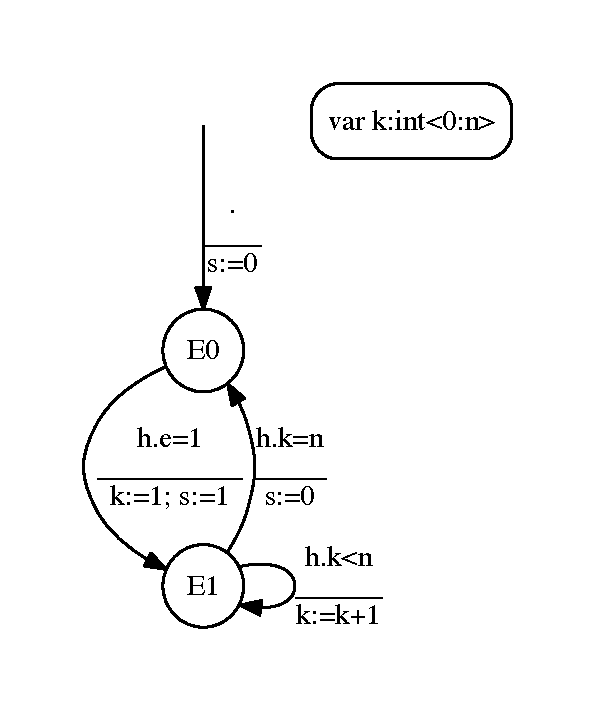
\includegraphics[height=6cm]{figs/gensig-model-mealy}
   \centering
  \caption{A Mealy-style reformulation of the model defined in Fig.~\ref{fig:rfsm-gensig-model}}
  \label{fig:rfsm-gensig-mealy}
\end{figure}

\begin{lstlisting}[language=Rfsm,frame=single,numbers=left,caption=Transcription in RFSM of the
  model given in Fig.~\ref{fig:rfsm-gensig-mealy},label={lst:rfsm-gensig-mealy},float]
fsm model gensig <n: int> (
  in h: event,
  in e: bool,
  out s: bool)
{
@\label{gensigm-1}@  states: E0, E1;
  vars: k: int<0:n>;
  trans:
@\label{gensigm-2a}@  | E0 -> E1 on h when e=1 with k:=1, s:=1
  | E1 -> E1 on h when k<n with k:=k+1
@\label{gensigm-2b}@  | E1 -> E0 on h when k=n, s:=0
  itrans:
@\label{gensigm-3}@  | -> E0 with s:=0
}
\end{lstlisting}

\medskip \textbf{Note}. An option of the \texttt{rfsmc} compiler (\verb|-normalize|) allows to
automatically transform a Moore-style description into a Mealy-style one.
% This option is
% automatically inserted when simulating a system\footnote{\emph{I.e.} simulation is always performed
%   on Mealy-style FSMs.}. 


%%% Local Variables: 
%%% mode: latex
%%% TeX-master: "rfsm"
%%% End: 
   
\chapter{Using the RFSM compiler}
\label{cha:rfsmc}

The RFSM compiler can be used to
\begin{itemize}
\item produce graphical representations of FSM models and programs (using the \verb|.dot| format),
\item simulate programs, generating execution traces (\verb|.vcd| format),
\item generate C, SystemC or VHDL code from FSM models and programs.
\end{itemize}

This chapter describes how to invoke compiler on the command-line. On Unix systems, this is
done from a terminal running a shell interpreter. On Windows, from an MSYS or Cygwin
terminal.

\medskip
The compiler is invoked with a command like :

%rfsmc [options] file\textsubscript{1} ... file\textsubscript{n}
\begin{FVerbatim}[commandchars=\\\{\}]
rfsmc [options] \emph{source_files}
\end{FVerbatim}

\medskip
There must be at least one source file. If several are given, all happens as if a single one,
obtained by concatening all of them, in the given order, was used. 

\medskip
The complete set of options is described in App.~\ref{cha:compiler-options}.

\medskip
The set of generated files depends on the selected target. The output file \texttt{rfsm.output}
contains the list of the generated file.

\section{Generating graphical representations}
\label{sec:gener-graph-repr}

%rfsmc -dot f\textsubscript{1}.fsm ... f\textsubscript{n}.fsm
\begin{FVerbatim}[commandchars=\\\{\}]
rfsmc [-options] -dot \emph{source_files}
\end{FVerbatim}

The previous command generates a graphical representation of each FSM model 
contained in the given source file(s). If the source file(s) contain(s) FSM instances, involving global IOs
and shared objects, it also generates a graphical representation of the the corresponding system. 

The graphical representations use the \verb|.dot| format and can be viewed
with the \texttt{Graphviz} suite of tools\footnote{Available freely from
  \texttt{http://www.graphviz.org}.}.

The representation for the FSM model \verb|m| is generated in file \verb|m.dot|. When generated, the representation
for the system is written in file \verb|main.dot| by default. The name of this file can be changed
with the \verb|-main| option.

By default, the generated \verb|.dot| files are written in the current directory. This can be changed with the
\verb|-target_dir| option.

\section{Running the simulator}
\label{sec:running-simulator}

\begin{FVerbatim}[commandchars=\\\{\}]
rfsmc [-options] -sim \emph{source_files}
\end{FVerbatim}

The previous command runs simulator on the program described in the given source files, writing
an execution trace in VCD (Value Change Dump) format.

The generated \verb|.vcd| file can be viewed using a VCD visualizing application such as
\verb|gtkwave|\footnote{gtkwave.sourceforge.net}.

By default, the VCD file is named \verb|main.vcd|. This name can be changed using the \verb|-main| option.

By default, the VCD file is written in the current directory. This can be changed with the
\verb|-target_dir| option.

\section{Generating C code}
\label{sec:gener-c-code}

\begin{FVerbatim}[commandchars=\\\{\}]
rfsmc [-options] -ctask \emph{source_files}
\end{FVerbatim}

For each FSM model \verb|m| contained in the listed source file(s), the previous command generates a file
\verb|m.c| containing a C-based implementation of the corresponding behavior.

By default, the generated code is written in the current directory. This can be changed with the
\verb|-target_dir| option.

\section{Generating SystemC code}
\label{sec:gener-syst-code}

\begin{FVerbatim}[commandchars=\\\{\}]
rfsmc [-options] -systemc \emph{source_files}
\end{FVerbatim}

If the source file(s) only contain(s) FSM \emph{models}, then, for each listed FSM model \texttt{m}, 
the previous command generates a pair of files \verb|m.h| and \verb|m.cpp| containing the
  interface and implementation of the SystemC module implementing this model.

\medskip
If the source file(s) contain(s) FSM \emph{instances}, involving global IOs
and shared objects, it generates
\begin{itemize}
\item for each FSM instance \verb|m|, a pair of files \verb|m.h| and \verb|m.cpp| containing the
  interface and implementation of the SystemC module implementing this instance,
\item for each global input \verb|i|, a pair of files \verb|inp_i.h|
  and \verb|inp_i.cpp| containing the interface and implementation of the SystemC module describing
  this input (generating the associated stimuli, in particular),
\item a file \verb|main.cpp| containing the description of the \emph{testbench} for simulating the
  program.
\end{itemize}

The name of the file containing the \emph{testbench} can be changed with the \verb|main| option.

\medskip
By default, the generated code is written in the current directory. This can be changed with the
\verb|-target_dir| option.

\medskip Simulation itself is performed by compiling the generated code and running the executable,
using the standard SystemC toolchain.  In order to simplify this, the RFSM compiler also generates a
customized \emph{Makefile} so that compiling and running the code generated by the SystemC backend
can be performed by simply invoking \verb|make|. For this, the compiler simply needs to know where
to find the predefined template from which this \emph{Makefile} is built. This is achieved by using
the \verb|-lib| option when invoking the compiler. For example, provided that RFSM has been
installed in directory \verb|/usr/local/rfsm|, the following command

\begin{FVerbatim}[commandchars=\\\{\}]
rsfmc -systemc -lib /usr/local/rfsm/lib -target_dir ./systemc \emph{source_file(s)}
\end{FVerbatim}

will write in directory \verb|./systemc| the generated source files and the corresponding
\verb|Makefile|. Compiling these files and running the resulting application is then simply achieved
by typing

\begin{verbatim}
cd ./systemc
make 
\end{verbatim}

\medskip
\textbf{Note}. The generated \emph{Makefile} uses platform-specific definitions which have been
written in a file named \verb|platform| located in RSFM library directory
(\verb|/usr/local/rfsm/lib/etc/plaform| in the example above). This file is generated by
the installation process from the values given to the \verb|configure| script. Depending on your
local SystemC installation, some definitions given in the \verb|platform| file may have to be
adusted.

\section{Generating VHDL code}
\label{sec:generating-vhdl-code}

\begin{FVerbatim}[commandchars=\\\{\}]
rfsmc [-options] -vhdl \emph{source_files}
\end{FVerbatim}

If the source file(s) only contain(s) FSM \emph{models}, then, for each listed FSM model \texttt{m}, 
the previous command generates file \verb|m.vhd| containing the entity and architecture describing
this model.

\medskip
If the source file(s) contain(s) FSM \emph{instances}, involving global IOs
and shared objects, it generates
\begin{itemize}
\item for each FSM instance \verb|m|, a file \verb|m.vhd| containing an entity and architecture
  description for this instance,
\item a file \verb|main_top.vhd| containing the description of the \emph{top level} model of the
  system,
\item a file \verb|main_tb.vhd|containing the description of the \emph{testbench} for
  simulating the system.
\end{itemize}

\medskip The name of the files containing the \emph{top level} description \emph{testbench} can be
changed with the \verb|main| option.

\medskip
By default, the generated code is written in the current directory. This can be changed with the
\verb|-target_dir| option.

\medskip
The produced files can then compiled, simulated and synthetized using a standard VHDL
toolchain\footnote{We use GHDL for simulation and Altera/Quartus for synthesis.}.

\medskip
As for the SystemC backend, the RFSM compiler simplifies the compilation and simulation of the
generated code by also generating a dedicated \emph{Makefile}. For example,
and, again, provided that RFSM has been installed in directory \verb|/usr/local/rfsm|, the following
command

\begin{FVerbatim}[commandchars=\\\{\}]
rsfmc -vhdl -lib /usr/local/rfsm/lib -target_dir ./vhdl \emph{source_file(s)}
\end{FVerbatim}

will write in directory \verb|./vhdl| the generated source files and the corresponding
\verb|Makefile|. Compiling these files and running the resulting application is then simply achieved
by typing

\begin{verbatim}
cd ./vhdl
make 
\end{verbatim}

\section{Using \texttt{rfsmmake}}
\label{sec:rfsmmake}

The current distribution provides a script named \verb|rfsmmake| aiming at easing the use of the
RSFM compiler in a command line environment. With this tool, the only thing required is to write a
small \emph{project description} (\verb|.pro| file\footnote{The \texttt{.pro} file is also used by
  the GUI described in chapter~\ref{cha:gui}.}). Invoking \verb|rfsmmake| will then
automatically build a top-level \emph{Makefile} which can be used to invoke the compiler, generate
code and exploit the generated products.

Suppose, for instance, that the application is made of two source files, \verb|foo.fsm|, containing the FSM model(s), and
\verb|main.fsm|, containing the global declarations and FSM instanciations (the so-called
\emph{testbench}). Writing the following lines in file \verb|main.pro|

\begin{lstlisting}[language=make,frame=single]
SRCS=foo.fsm main.fsm
DOT_OPTS= ...
SIM_OPTS= ...
SYSTEMC_OPTS= ...
VHDL_OPTS= ...
\end{lstlisting}

\noindent
and invoking

\begin{verbatim}
rfsmmake main.pro
\end{verbatim}

\noindent
will generate a file \verb|Makefile| in the current directory. 
Then, simply typing\footnote{Please refer to the generated \emph{Makefile} for
  a complete list of targets.}
  \begin{itemize}
  \item \verb|make dot| will generate the \verb|.dot| and lauch the corresponding viewer,
  \item \verb|make sim.run| to run the simulation using the interpreter (\verb|make sim.show| to display results),
  \item \verb|make ctask.code| will invoke the C backend C and generate the corresponding code,
  \item \verb|make systemc.code| will invoke the SystemC backend  and generate the corresponding code,
  \item \verb|make systemc.run| will invoke the SystemC backend, generate the corresponding
    code, compile it and run the corresponding simulation,
  \item \verb|make vhdl.code| will invoke the VHDL backend  and generate the corresponding code,
  \item \verb|make vhdl.run| will invoke the VHDL backend, generate the corresponding
    code, compile it and run the corresponding simulation,
  \item \verb|make sim.show| (resp \verb|make systemc.show| and \verb|make vhdl.show|) will display
    the simulation traces generated by the interpreter (resp. SystemC and VHDL simulation).
  \end{itemize}


%%% Local Variables: 
%%% mode: latex
%%% TeX-master: "rfsm"
%%% End: 

\chapter*{Appendix A - Formal syntax of RFSM programs}
\label{cha:bnf}

This appendix gives a BNF definition of the concrete syntax RFSM programs.

\medskip
The meta-syntax is conventional. Keywords are written in \textbf{boldface}.  Non-terminals are
enclosed in angle brackets ({\tt <} \ldots {\tt >}).  Vertical bars ({\tt |}) indicate
alternatives.  Constructs enclosed in non-bold brackets ({\tt [} \ldots {\tt ]}) are optional.
The notation $E^*$ (resp $E^+$) means zero (resp one) or more repetitions of $E$, separated by spaces.
The notation $E^*_x$ (resp $E^+_x$) means zero (resp one) or more repetitions of $E$, separated by
symbol $x$. Terminals \verb|lid| and \verb|uid| respectively designate identifiers
starting with a lowercase and uppercase letter. 

\documentclass[11pt,a4paper]{article}

\title{Links Grammar}
\date{}

\usepackage{shortvrb}
\usepackage{longtable}
\begin{document}
\maketitle
\tableofcontents

\begingroup
\catcode`<=\active
\catcode`>=\active
\catcode`!=\active
\gdef\setupgrammardefs{
  \catcode`\<=\active \def <{$\langle$}
  \catcode`\>=\active \def >{$\rangle$}
  \catcode`\!=\active \def !{$\mid$}
}
\endgroup

\newenvironment{grammar}{
  \setupgrammardefs
  \begin{itshape}
    \begin{small}
      \MakeShortVerb{\'}
\begin{longtable}{llll}
}{
\end{longtable}
    \DeleteShortVerb{\'}
    \end{small}
  \end{itshape}
}

\section{Grammar for patterns}

\begin{grammar}
pattern &::=& as-pattern < ':' primary-datatype >  \\
\\
as-pattern &::=& cons-pattern < 'as' 'VARIABLE' >  \\
\\
cons-pattern &::=& constructor-pattern < '::' cons-pattern > \\
\\
constructor-pattern &::=& primary-pattern \\
&&                        'CONSTRUCTOR' < parenthesized-pattern > \\
\\
parenthesized-pattern &::=& '(' < pattern < ',' patterns >> ) \\
&&                         '(' labeled-patterns < ! pattern > ) \\
\\
primary-pattern &::=& 'VARIABLE' \\
&&                     '_' \\
&&                     special-constant \\
&&                     '[' < patterns > ']' \\
&&                     parenthesized-pattern \\
\\
patterns &::=& pattern < ',' patterns > \\
\\
labeled-patterns &::=& record-label = pattern < , labeled-patterns > \\
\end{grammar}

\section{Grammar for types}

\begin{grammar}
datatype &::=& mu-datatype < '->' datatype > \\
&&             mu-datatype < '-{' datatype '}->' datatype > \\
\\
mu-datatype &::=& 'mu' 'VARIABLE' '.' mu-datatype \\
&&                primary-datatype \\
\\
primary-datatype &::=& '(' datatype ')' \\
&&                     '(' < datatype , datatypes > ')' \\
&&                     '(' fields ')' \\
&&                     '{' 'VARIABLE' '}' \\
&&                     TableHandle '(' datatype ',' datatype ')' \\
&&                     '[[' < vfields > ']]' \\
&&                     '[' datatype ']' \\
&&                     'VARIABLE' \\
&&                     'QUOTE' 'VARIABLE' \\
&&                     'CONSTRUCTOR' '('< primary-datatype-list >')' \\
\\
primary-datatype-list &::=& primary-datatype < ',' primary-datatype-list > \\
\\
vfields &::=&  'VARIABLE'  \\
&&             'CONSTRUCTOR' < ':' spec >  < ! vfields > \\
\\
datatypes &::=& datatype < ',' datatypes > \\
\\
tfields &::=& fields \\
&&            'VARIABLE' \\
\\
fields &::=&  field < ! 'VARIABLE' >  \\
&&            field ',' fields \\
\\
spec &::=& '-' \\
&&         datatype \\
\\
field &::=& record-label ':' spec \\
\end{grammar}

\section{Grammar for regular expressions}

\begin{grammar}
regex &::=&  '/' < regex-pattern-sequence >  '/' \\
\\
regex-pattern &::=& '[' 'REGEXCHAR' '-' 'REGEXCHAR' ']'  \\
&&                  '.' \\
&&                  'REGEXCHAR' \\
&&                  '(' regex-pattern-sequence ')' \\
&&                  regex-pattern repeat-op \\
&&                  block \\
\\
repeat-op &::=& '*' \\
&&              '+' \\
&&              '?' \\
\\
regex-pattern-sequence &::=& regex-pattern < regex-pattern-sequence > \\
\end{grammar}

\section{Grammar for expressions}

\begin{grammar}
location &::=& 'server' \\
&&             'client' \\
&&             'native' \\
\\
special-constant &::=& 'UINTEGER' \\
&&                     'UFLOAT' \\
&&                     'true' \\
&&                     'false' \\
&&                     'STRING' \\
&&                     'CHAR' \\
\\
atomic-expression &::=& 'VARIABLE' \\
&&                      special-constant \\
&&                      parenthesized-expression \\
\\
primary-expression &::=& atomic-expression \\
&&                       '[' < exps > ']' \\
&&                       xml-forest \\
&&                       'fun' arg-list block \\
\\
constructor-expression &::=& 'CONSTRUCTOR' < parenthesized-expression > \\
\\
parenthesized-expression &::=&  '(' binop ')' \\
&&                              '(' '.' record-label ')' \\
&&                              '(' exps ')' \\
&&                              '(' exp 'with' labeled-exps ')' \\
&&                              '(' labeled-exps < ! exp > ')' \\
\\
binop &::=& '-' \\
&&          '-.' \\
&&          infix-op \\
\\
infix-op &::=&  '`' 'VARIABLE' '`' \\
&&              'SYMBOL' \\
\\
postfix-expression &::=&  primary-expression \\
&&                        block \\
&&                        'query' block \\
&&                        'spawn' block \\
&&                        'spawnWait' block \\
&&                        postfix-expression '.' record-label \\
&&                        postfix-expression '(' < exps > ')' \\
\\
exps &::=& exp < ',' exps >  \\
\\
unary-expression &::=& '-' unary-expression \\
&&                     '-.' unary-expression \\
&&                     postfix-expression \\
&&                     constructor-expression \\
\\
infix-expression &::=& unary-expression \\
&&                     infix-expression infix-op infix-expression \\
&&                     infix-expression '~' regex \\
\\
logical-expression &::=& infix-expression \\
&&                       logical-expression !! infix-expression \\
&&                       logical-expression '&&' infix-expression \\
\\
typed-expression &::=& logical-expression < ':' datatype > \\
\\
db-expression &::=& typed-expression \\
&&                  'insert' exp 'values' exp \\
&&                  'delete' '(' table-generator ')' < where >  \\
&&                  'update' '(' table-generator ')' < where > 'set' '(' labeled-exps ')' \\
\\
where &::=& 'where' '(' exp ')' \\
\\
xml-forest &::=& xml-tree \\
&&               xml-tree xml-forest \\
\\
xmlid &::=& 'VARIABLE' \\
\\
attr-list &::=& xmlid = '"' < attr-val > '"' < attr-list >  \\
\\
attr-val &::=& block < attr-val > \\
&&             string < attr-val >  \\
\\
xml-tree &::=& '<' 'QNAME' < attr-list > '/>' \\
&&             '<' 'QNAME' < attr-list > '>' < xml-contents-list > '</' 'QNAME' '>' \\
\\
xml-contents-list &::=& xml-contents < xml-contents-list > \\
\\
xml-contents &::=& block \\
&&                 'CDATA' \\
&&                 '{' logical-expression '->' pattern '}' \\
&&                 xml-tree \\
\\
conditional-expression &::=& db-expression \\
&&                           'if' '(' exp ')' exp 'else' exp \\
\\
cases &::=& 'case' pattern '->' block-contents < cases >  \\
\\
case-expression &::=&  conditional-expression \\
&&                     'switch' '(' exp ')' '{' < cases > '}' \\
&&                     'receive' '{' < cases > '}' \\
\\
iteration-expression &::=& case-expression \\
&&                         'for' '(' generator ')' < where > < 'orderby' '(' exp ')' > exp \\
\\
generator &::=&  list-generator \\
&&               table-generator \\
\\
list-generator  &::=&  pattern '<-' exp \\
table-generator &::=& pattern '<--' exp \\
\\
escape-expression &::=& iteration-expression \\
&&                      'escape' 'VARIABLE' 'in' postfix-expression \\
\\
formlet-expression &::=& escape-expression \\
&&                       'formlet' xml-contents-list 'yields' exp \\
\\
table-expression &::=&  formlet-expression \\
&&                      'table' exp 'with' datatype < 'where' constraints > 'from' exp \\
\\
constraints &::=& record-label 'readonly' < ',' constraints > \\
\\
arg-list &::=& parenthesized-pattern < arg-list >  \\
\\
binding &::=& 'var' pattern '=' exp ';' \\
&&            exp ';' \\
&&            'fun' 'VARIABLE' arg-list block \\
\\
bindings &::=& < bindings > binding \\
\\
block &::=& '{' block-contents '}' \\
\\
block-contents &::=& < bindings > < exp > < ';' >  \\
\\
labeled-exps &::=& record-label '=' exp < ',' labeled-exps > \\
\\
exp &::=& table-expression \\
&&        'database' atomic-expression < atomic-expression > < atomic-expression >  \\
\end{grammar} 

\section{Grammar for files and declarations}

\begin{grammar}
file &::=& < declarations > < exp > \\
\\
declarations &::=& < declarations > declaration \\
\\
declaration &::=& fixity 'UINTEGER' infix-op ';' \\
&&               'typename' 'CONSTRUCTOR' < '(' typevars ')' > '=' datatype ';' \\
&&                < signature > toplevel-binding \\
\\
typevars &::=& 'VARIABLE' < ',' typevars > \\
\\
toplevel-binding &::=& 'var' pattern perhaps-location '=' exp ';' \\
&&                     'fun' 'VARIABLE' arg-list < location > block < ';' > \\
&&                     'fun' pattern infix-op pattern < location > block < ';' > \\
\\
fixity &::=& 'infix' \\
&&           'infixl' \\
&&           'infixr' \\
\\
signature &::=& 'sig' 'VARIABLE' ':' datatype \\
&&              'sig' infix-op ':' datatype \\
\end{grammar} 

% prefix and postfix operators, alien not documented

\section{Terminals} 
 
\MakeShortVerb{\'} 
 
The meaning of non-literal terminals, which occur in uppercase in the 
grammar, is as follows: 
 
Identifier character an uppercase or lowercase letter, a digit, or
underscore (\texttt{\_}).  Then a 'CONSTRUCTOR' is a non-empty
sequence of identifiers starting with an uppercase letter and a
'VARIABLE' is a non-empty sequence of identifiers starting with a
lowercase letter.  A 'UINTEGER' is either '0' or a non-empty sequence
of digits starting with a non-zero digit.  A 'SYMBOL' is a non-empty
sequence of non-identifier characters (e.g. '++' or \texttt{\$@}).  A
'REGEXCHAR' is a character not otherwise employed in the grammar for
regular expressions.  A 'QNAME' is a non-empty sequence of identifier
characters and colons; the first character may not be a colon.  A
'UFLOAT' consists of a 'UINTEGER', a dot ('.'), a possibly-empty
sequence of digits and an optional exponent part consisting of the
letter 'e', an optional minus ('-'), and a 'UINTEGER'.  'QUOTE'
represents the single quote character, \verb$'$.
 
An escape character is a backslash ('\') followed by three octal 
digits, or by an uppercase or lowercase 'x' followed by two 
hexadecimal digits.  A 'STRING' consists of a possibly-empty sequence of 
characters (other than '"'), escape characters and the sequence '\"' 
between double quotes ('"').  A 'CHAR' consists of a character other than 
an escape character or the character \verb$'$ between single quotes (\verb$'$). 
'CDATA' is a non-empty sequence of characters other than '{','}','<' or '&'. 
 
\DeleteShortVerb{\'} 
 
 
\end{document} 


%%% Local Variables:
%%% mode: latex
%%% TeX-master: "rfsm"
%%% End:

\chapter*{Appendix B - Compiler options}
\label{cha:compiler-options}

Compiler usage : \verb|rfsmc [options...] files|

\medskip
\begin{tabular}[c]{ll}
-lib & set location of the support library (default: <opam\_prefix>/share/rfsm)\\
-main & set prefix for the generated main files\\
-dump\_static & dump static representation of model(s)/program to stdout\\
-target\_dir & set target directory (default: .)\\
-dot & generate .dot representation of model(s)/program\\
-ctask & generate CTask code\\
-systemc & generate SystemC code\\
-vhdl & generate VHDL code\\
-sim & run simulation (generating .vcd file)\\
-version & print version of the compiler and quit\\
-dot\_no\_captions & Remove captions in .dot representation(s)\\
-dot\_actions\_nl & write actions with with a separating newline\\
-trace & set trace level for simulation (default: 0)\\
-synchronous\_actions & interpret actions synchronously\\
-normalize & move output assignations from states to transitions\\
-sc\_time\_unit & set time unit for the SystemC test-bench (default: SC\_NS)\\
-sc\_trace & set trace mode for SystemC backend (default: false)\\
-stop\_time & set stop time for the SystemC and VHDL test-bench (default: 100)\\
-sc\_double\_float & implement float type as C++ double instead of float (default: false)\\
-vhdl\_trace & set trace mode for VHDL backend (default: false)\\
-vhdl\_time\_unit & set time unit for the VHDL test-bench\\
-vhdl\_ev\_duration & set duration of event signals (default: 1 ns)\\
-vhdl\_rst\_duration & set duration of reset signals (default: 1 ns)\\
-vhdl\_numeric\_std & translate integers as numeric\_std [un]signed (default: false)\\
-vhdl\_bool\_as\_bool & translate all booleans as boolean (default: false)\\
-vhdl\_dump\_ghw & make GHDL generate trace files in .ghw format instead of .vcd\\
-old\_syntax & use old (pre-1.5) syntax\\
-transl\_syntax & convert old syntax to new syntax\\

\end{tabular}

\normalsize

%%% Local Variables: 
%%% mode: latex
%%% TeX-master: "rfsm"
%%% End: 

\chapter*{Appendix C1 - Example of generated C code}  
\label{cha:ex1-c}

This is the code generated from program given in Listing~\ref{lst:rfsm-gensig} 

\begin{lstlisting}[language=ctask,frame=single,numbers=none,basicstyle=\small]
task g(
  in event h;
  in bool e;
 out bool s;
  )
{
  int k;
  enum {E0,E1} state = E0;
  while ( 1 ) {
    switch ( state ) {
    case E1:
      s = true;
      wait_ev(h);
      if ( k<4 ) {
        k=k+1;
        }
      else if ( k==4 ) {
        state = E0;
        }
      break;
    case E0:
      s = false;
      wait_ev(h);
      if ( e==true ) {
        k=1;
        state = E1;
        }
      break;
    }
  }
};
\end{lstlisting}
%%% Local Variables: 
%%% mode: latex
%%% TeX-master: "rfsm"
%%% End: 

\chapter*{Appendix C1 - Example of generated SystemC code}  
\label{cha:ex1-systemc}

This is the code generated from program given in Listing~\ref{lst:rfsm-gensig} 

\begin{lstlisting}[language=systemc,frame=single,numbers=none,basicstyle=\small,caption=File g4.h]
#include "systemc.h"

SC_MODULE(G)
{
  // Types
  typedef enum { E0, E1 } t_state;
  // IOs
  sc_in<bool> h;
  sc_in<sc_uint<1> > e;
  sc_out<sc_uint<1> > s;
  // Constants
  static const int n = 4;
  // Local variables
  t_state state;
  sc_uint<3>  k;

  void react();

  SC_CTOR(G) {
    SC_THREAD(react);
    }
};
\end{lstlisting}

\begin{lstlisting}[language=systemc,frame=single,numbers=none,basicstyle=\small,caption=File g.cpp]
#include "g.h"
#include "rfsm.h"

void G::react()
{
  state = E0;
  while ( 1 ) {
    switch ( state ) {
    case E1:
      s.write(1);
      wait(h.posedge_event());
      if ( k<4 ) {
        k=k+1;
        }
      else if ( k==4 ) {
        state = E0;
        }
      wait(SC_ZERO_TIME);
      break;
    case E0:
      s.write(0);
      wait(h.posedge_event());
      if ( e.read()==true ) {
        k=1;
        state = E1;
        }
      wait(SC_ZERO_TIME);
      break;
    }
  }
};
\end{lstlisting}

\begin{lstlisting}[language=systemc,frame=single,numbers=none,basicstyle=\small,caption=File inp_H.h]
#include "systemc.h"

SC_MODULE(Inp_H)
{
  // Output
  sc_out<bool> H;

  void gen();

  SC_CTOR(Inp_H) {
    SC_THREAD(gen);
    }
};
\end{lstlisting}

\begin{lstlisting}[language=systemc,frame=single,numbers=none,basicstyle=\small,caption=File inp_H.cpp]
#include "inp_H.h"
#include "rfsm.h"

typedef struct { int period; int t1; int t2; } _periodic_t;

static _periodic_t _clk = { 10, 0, 80 };

void Inp_H::gen()
{
  int _t=0;
  wait(_clk.t1, SC_NS);
  notify_ev(H,"H");
  _t = _clk.t1;
  while ( _t <= _clk.t2 ) {
    wait(_clk.period, SC_NS);
    notify_ev(H,"H");
    _t += _clk.period;
    }
};
\end{lstlisting}

\begin{lstlisting}[language=systemc,frame=single,numbers=none,basicstyle=\small,caption=File inp_E.h]
#include "systemc.h"

SC_MODULE(Inp_E)
{
  // Output
  sc_out<sc_uint<1> > E;

  void gen();

  SC_CTOR(Inp_E) {
    SC_THREAD(gen);
    }
};
\end{lstlisting}

\begin{lstlisting}[language=systemc,frame=single,numbers=none,basicstyle=\small,caption=File inp_E.cpp]
#include "inp_E.h"
#include "rfsm.h"

typedef struct { int date; int val; } _vc_t;
static _vc_t _vcs[3] = { {0,0}, {25,1}, {35,0} };

void Inp_E::gen()
{
  int _i=0, _t=0;
  while ( _i < 3 ) {
    wait(_vcs[_i].date-_t, SC_NS);
    E = _vcs[_i].val;
    _t = _vcs[_i].date;
    _i++;
    }
};
\end{lstlisting}

\begin{lstlisting}[language=systemc,frame=single,numbers=none,basicstyle=\small,caption=File tb.cpp]
#include "systemc.h"
#include "rfsm.h"
#include "inp_E.h"
#include "inp_H.h"
#include "g.h"

int sc_main(int argc, char *argv[])
{
  sc_signal<sc_uint<1> > E;
  sc_signal<bool> H;
  sc_signal<sc_uint<1> > S;
  sc_trace_file *trace_file;
  trace_file = sc_create_vcd_trace_file ("tb");
  sc_trace(trace_file, E, "E");
  sc_trace(trace_file, H, "H");
  sc_trace(trace_file, S, "S");

  Inp_E Inp_E("Inp_E");
  Inp_E(E);
  Inp_H Inp_H("Inp_H");
  Inp_H(H);

  G g("g");
  g(H,E,S);

  sc_start(100, SC_NS);

  sc_close_vcd_trace_file (trace_file);

  return EXIT_SUCCESS;
}
\end{lstlisting}

%%% Local Variables: 
%%% mode: latex
%%% TeX-master: "rfsm"
%%% End: 

\chapter*{Appendix C3 - Example of generated VHDL code}  
\label{cha:ex1-vhdl}

This is the code generated from program given in Listing~\ref{lst:rfsm-gensig} 

\begin{lstlisting}[language=VHDL,frame=single,numbers=none,basicstyle=\small,caption=File g.vhd]
library ieee;
use ieee.std_logic_1164.all;
use ieee.numeric_std.all;
library rfsm;
use rfsm.core.all;

entity g is
  port(
        h: in std_logic;
        e: in std_logic;
        s: out std_logic;
        rst: in std_logic
        );
end g;

architecture RTL of g is
  type t_state is ( E0, E1 );
  signal state: t_state;
  signal k: unsigned(2 downto 0);
begin
  process(rst, h)
  begin
    if ( rst='1' ) then
      state <= E0;
      s <= '0';
    elsif rising_edge(h) then 
      case state is
      when E1 =>
        if ( k<to_unsigned(4,3) ) then
          k <= k+to_unsigned(1,3);
        elsif  ( k = to_unsigned(4,3) ) then
          s <= '0';
          state <= E0;
        end if;
      when E0 =>
        if ( e = '1' ) then
          k <= to_unsigned(1,3);
          s <= '1';
          state <= E1;
        end if;
    end case;
    end if;
  end process;
end RTL;
\end{lstlisting}

\begin{lstlisting}[language=VHDL,frame=single,numbers=none,basicstyle=\small,caption=File tb.vhd]
library ieee;
use ieee.std_logic_1164.all;	   
use ieee.numeric_std.all;
library rfsm;
use rfsm.core.all;

entity tb is
end tb;

architecture Bench of tb is

component g 
  port(
        h: in std_logic;
        e: in std_logic;
        s: out std_logic;
        rst: in std_logic
        );
end component;

signal E: std_logic;
signal H: std_logic;
signal S: std_logic;
signal rst: std_logic;

begin

  inp_E: process
    type t_vc is record date: time; val: std_logic; end record;
    type t_vcs is array ( 0 to 2 ) of t_vc;
    constant vcs : t_vcs := ( (0 ns,'0'), (25 ns,'1'), (35 ns,'0') );
    variable i : natural := 0;
    variable t : time := 0 ns;
    begin
      for i in 0 to 2 loop
        wait for vcs(i).date-t;
        E <= vcs(i).val;
        t := vcs(i).date;
      end loop;
      wait;
  end process;
  inp_H: process
    type t_periodic is record period: time; t1: time; t2: time; end record;
    constant periodic : t_periodic := ( 9 ns, 0 ns, 80 ns );
    variable t : time := 0 ns;
    begin
      H <= '0';
      wait for periodic.t1;
      notify_ev(H,1 ns);
      while ( t < periodic.t2 ) loop
        wait for periodic.period;
        notify_ev(H,1 ns);
        t := t + periodic.period;
      end loop;
      wait;
  end process;

  U0: G port map(H,E,S,rst);

  process

  begin
    rst <= '1';
    wait for 1 ns;
    rst <= '0';
    wait for 100 ns;
    wait;

  end process;
end Bench;
\end{lstlisting}

%%% Local Variables: 
%%% mode: latex
%%% TeX-master: "rfsm"
%%% End: 


% \input{source}
% \input{biblio}

\bibliographystyle{plain}
\bibliography{rfsm}

\end{document}

%%% Local Variables:
%%% mode: latex
%%% TeX-master: t
%%% End:
